\chapter{\acl{FEC}}
\label{chap:forward_error_correction}

In the last chapters, we described the effect of temperature on \ac{BER} patterns and \ac{PRR}, without drafting any specific recommendations how to improve this loss of link quality.
\ac{FEC} is a well known technique to improve throughput in links of poor quality, however, once a \ac{ECC} and its parameters have been chosen, usually they remain static and do not change over time.
This means that for links where the quality is not stable over time, as in \acp{WSN}, the chosen \ac{ECC} incurs unneeded overhead in links with overal good link quality, and underperforms in links with poor quality.

We therefore wanted to investigate how using temperature as an indicator for adapting \ac{ECC} parameter can benefit \ac{PRR} and throughput and what improvements and limitations to expect.
In doing so, we are moving away from a macro-view of all influences on link quality to focus on the impact of temperature on \ac{FEC} on \emph{one} link at a time.

We extended the control software described in Section~\ref{sec:control_software} to encode messages to be sent and to decode received messages with an \ac{FEC} scheme.
The messages are logged in the same format, with the additional information of the FEC scheme and coding strength.
This allows us to reuse our existing evaluation software to easily map error-free \ac{PRR} to \emph{decoded} error-free \ac{PRR}.


\section{Choice of \acs{FEC} Scheme}

Choosing a coding scheme is not only a matter of its error correction capabilities, but also about the complexity of its coder and decoder, considering the tight computational resources of a \ac{WSN} mote.
Practical implementations are therefore limited to cyclic linear block coding, with the most widely used codes being binary \ac{BCH} and non-binary \ac{RS} codes, which can be combined with interleaving and code shortening~\cite{Liu1997}.
Furthermore, since data payload size is limited to 125 bytes by the \ac{MPDU}, of which we use 93 in our messages (with 80 bytes data), a low coding overhead among \ac{ECC}s with the same error correction capability is preferred.

A \ac{RS} code works over $m$-bit symbols, and is denoted as $RS(n, k)$, where $n$ is the number of $m$-bit symbols in a codeword, and $k$ the number of original $m$-bit data symbols.
This leaves $n-k$ parity $m$-bit symbols, as shown in Figure~\ref{fig:rs_codeword}.
The symbol size $m$ can be set to bit-level, byte-level or packet-level size. We will use byte-level ($m=8$) symbol sizes, since they are efficient to work with on a microcontroller.
A \ac{RS} decoder can correct up to $t=(n-k)/2$ symbol errors, and up to $2t$ erasures, if the positions of the symbol errors are known~\cite{Liu1997}.

Similarly, for symbol size $m \ge 3$ and symbol error occurance $t < 2^{m-1}$, a \ac{BCH} code encodes block lengths of $n = 2^m - 1$ bit with $n-k \le mt$ parity check bits by multiplication with a generator matrix, that contains a $n \times n$ identity and a $n \times (n-k)$ binary matrix.
The decoder can construct a parity matrix using this information, which allows correction of $t$-bit errors, depending on the parameters chosen~\cite{Liu1997}.

Since the \ac{RS} scheme works by correcting entire $m$-bit symbols ($m=8$ for our case), burst errors up to $m$-bit in the same symbol require only correcting this specific symbol, while one-bit errors in many different symbols requires correcting all of these symbols.
\ac{RS} codes therefore perform better than \ac{BCH} codes in conditions with burst errors as described in Subsection~\ref{subsec:effects_of_board_layout}, but worse if same amount of bit errors are spread around more independently.
The performance of \ac{BCH} codes can be improved however, by interleaving symbols after encoding before transmission, which spreads out burst errors into many single bit errors.
However, \ac{BCH} codes generally require more transmission overhead compared with \ac{RS} codes of the same error correction capabilities.

\ac{RS} codes are well understood coding schemes, which have been compared to many others.
By using \ac{RS} codes as a benchmark we enable application of our results onto other, more complex schemes, such as a modified Turbo Code~\cite{Schmidt2009} and \ac{LDPC}~\cite{Sartipi2004} codes, which have been shown to outperform cyclic linear block codes.
Furthermore, a \ac{RS} implementation optimized for TinyOS, called TinyRS~\cite{Liang2010}, exists and therefore does not need to be implemented manually.

\begin{figure}[t]
	\begin{tikzpicture}[>=stealth', |<->|, very thick, shorten <=-0.5pt, shorten >=-0.5pt]

		\draw[thick] (0,-0.35) rectangle (10,0.35) node[midway] {Data};
		\draw[fill=slightgray, thick] (10,-0.35) rectangle (15,0.35) node[midway] {Parity};

		\draw (0,0.7) -- (10,0.7) node[midway, above] {$k$};
		\draw (10,0.7) -- (15,0.7) node[midway, above] {$80 - k$};
		\draw (0,-0.7) -- (15,-0.7) node[midway, below] {$n = 80$};

	\end{tikzpicture}
	\caption{Structure of an $RS(n, k)$ encoded codeword of 80 bytes length.}
	\label{fig:rs_codeword}
\end{figure}

\section{\acs{RS} Scheme Simulation}
\label{sec:fec_scheme_simulation}

To be able to investigate the effect that different \ac{RS} coding strengths have on decoded \ac{PRR}, we needed a way to compare experiment results.
Due to the difficulty of recreating the \emph{exact} same conditions for several series of real world experiments, we chose to create and use a trace-based simulator to apply the bit error patterns of an original experiment onto several new $RS(n, k)$ encoded random payloads.

By interpreting the $RS(80, 70)$ encoded random payload as pseudo-random in the context of Section~\ref{sec:packet_reception_rate}, we made dual-use of that experiment.
This allows us an in-depth description of the link conditions onto which we built our analysis of \ac{RS} performance.

We will next describe how we use the raw data of this experiment as an input for our simulation, by extracting its \ac{BER} patterns and applying them onto new payload, and discuss accuracy and limitations.

\subsection{Design}

The simulator re-runs an original experiment message-by-message over its log, and outputs a new one.
We only simulate \ac{BER} patterns, all other properties of the link, such as link qualifiers, temperature, transmission power, are copied from the original link, as visualized in Figure~\ref{fig:simulator_design}.
In addition, if a message was not received by a receiver, we simply preserve it as a timeout, to make later comparison of the simulated results with the real experiments much easier.

Our simulator also works with experiments where a transmitted message is received by multiple receivers as in Section~\ref{subsec:effects_of_board_layout}.
In such a case, the simulator will apply its algorithm to every received message.

\begin{figure}[t]
	\centering
	\tikzset{
	    %Define standard arrow tip
	    >=stealth',
	    %Define style for boxes
	    punkt/.style={
	           rectangle,
	           rounded corners,
	           draw=black, very thick,
	           text width=2cm,
	           minimum height=1cm,
	           text centered},
	    % Define arrow style
	    pil/.style={
	           ->,
	           very thick,
	           shorten <=2pt,
	           shorten >=2pt,}
	}
	\begin{tikzpicture}

		\fill[color=slightgray, rounded corners] (1.4,-4) rectangle (11,-2);

		\node[punkt] (input) {Input Message(s)};
 		\node[punkt, right=0.8cm of input] (parser) {Parser};
 		\node[punkt, right=3.85cm of parser] (formatter) {Formatter};
 		\node[punkt, right=0.8cm of formatter] (output) {Output Message};

 		\node[punkt, below=2cm of parser, fill=white] (analyzer) {Analyzer};
 		\node[punkt, below=2cm of formatter, fill=white] (corruptor) {Corrupter};
 		\node[right=0.85cm of corruptor] (payload) {New Payload};

 		\draw[pil] (input) -- (parser);
 		\draw[pil] (parser) -- (formatter) node[midway, below] {LQI, RSSI};
 		\path (parser) -- (formatter) node[midway, above] {Temperature};
 		\draw[pil] (formatter) -- (output);

 		\draw[pil] (parser) -- (analyzer) node[midway, left] {Original Payload(s)};
 		\draw[pil] (analyzer) -- (corruptor) node[midway, above] {BER pattern};
 		\draw[pil] (payload) -- (corruptor);
 		\draw[pil] (corruptor) -- (formatter) node[midway, right] {New Corrupted Payload};

 		\draw[pil] (input) edge[bend left=25] node[below]{Timeout} (output);

		% \draw (-1.2,-5) rectangle (13.8,1);
	\end{tikzpicture}
	\caption{Schematic design of our trace-based simulator: the payloads of multiple original messages can be analyzed to extract the \ac{BER} pattern, which is then applied to new payload.}
	\label{fig:simulator_design}
\end{figure}


\paragraph{Pattern Extraction}

Since we know that the \ac{BER} pattern is different for every of the 16 4-bit symbols, we need to generate a corruption probability for each bit within every symbol.
For that we sum up the bit errors per bit \emph{per symbol} for every original received message in the experiment in a corruption table.
The corruption table is then normalized for the occurrence of the respective symbol in the original message to yield a relative bit error occurrences \emph{per symbol} for this specific link.

This table can be averaged over several links using a sliding window, which reduces noise and increases the likelihood of seeing all symbols with their respective bit error patterns at least once.
This will create a corruption table of \emph{average} bit error probabilities per symbol over one or more messages.
We also average the distribution of bit error burst lengths over these messages in a burst error table.
Both the corruption and the burst error table will then be handed over to the corruption generator.

Since these tables are generated on-the-fly entirely from an experiment log, even the anomalous patterns described in Section~\ref{subsec:pattern_anomalies} can be extracted.

\paragraph{Pattern Application}

A corruption pattern is generated by randomly corrupting each new symbol with the probability defined in the bit error table.
This corruption pattern needs to be adapted for the burst error distribution of the original message by lengthening single bit errors accordingly.

The corruption sequence is applied to the new payload defined by us and written out as a new received message of the original link.

\paragraph{Limitations}

Since we map and apply bit error distribution \emph{per symbol}, every symbol must be available in the original payload at least once for this table to be complete.
Experiment logs with constant payload in which not every symbol is available should be avoided.
For random payload our message size of 93 bytes yields 186 symbols, for which it is unlikely to not see every 16 symbols at least once.

Another limitation is our modeling of the burst error distribution.
By ``simply'' applying the collected bit error table by symbol onto new payload, we are effectively interleaving the original burst errors and therefore obscuring this property of the original link.
With our simple simulation, we can only add burst errors to correct for relative occurrence compared to the original frame, but not willfully ``place'' these burst errors at the correct position to achieve the distinct burst error properties of the original link.

\subsection{Accuracy}
\label{subsec:simulation_accuracy}

To evaluate the performance of the simulator, we ran it on experiment traces containing constant payloads as well as $RS(80,70)$ encoded payloads.
By tuning the link input window size and the burst error generator, we were able to replicate similar enough bit error patterns for our purposes.
We found best accuracy with a window size of two messages.

\paragraph{Bit Error Distribution Patterns}

Figure~\ref{fig:8mote_xl_xor_simulation} and \ref{fig:8mote_s_simulation} show the bit error pattern resulting of simulating XL and S magnitudes of the experiment described in Subsection~\ref{subsec:effects_of_board_layout}.
Compared to the original patterns in Figure~\ref{fig:8mote_bit_errors}, the simulation generates a less noisy footprint with less amplitude, which makes the differences in symbols clearly visible.
This is, of course, due to the averaging during the symbol error construction that is accompanied with the smoothing of these values.

\paragraph{Burst Error Distribution}

The limitations of our burst error modeling clearly show in the burst error graph in Figure~\ref{fig:8mote_xl_burst_simulation} of the simulation. In comparison to Figure~\ref{fig:8mote_burst_error}, the simulated corruption does not exhibit the drop between 4/5-bit and 8/9-bit bursts and generates longer bursts more frequently.

\begin{figure}[t]
	\subfigure[Simulated XL bit error pattern.] {
		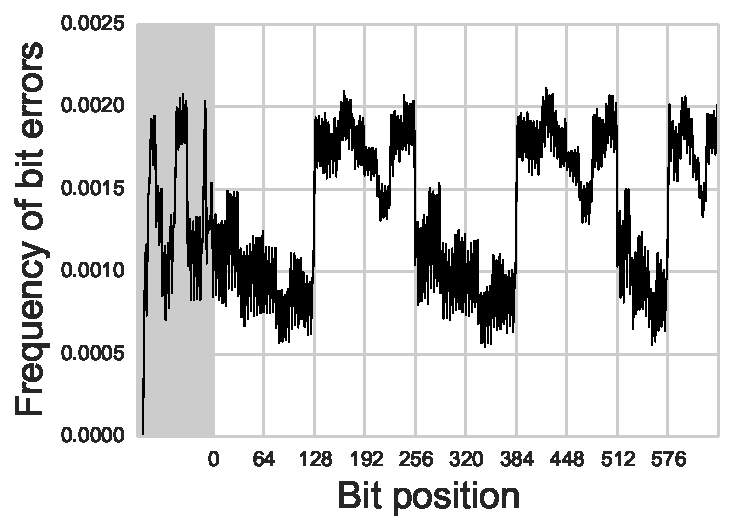
\includegraphics[width=0.475\columnwidth]{figures/8mote_0-5_xor_simulation}
		\label{fig:8mote_xl_xor_simulation}
	}
	\subfigure[Simulated S bit error pattern.] {
		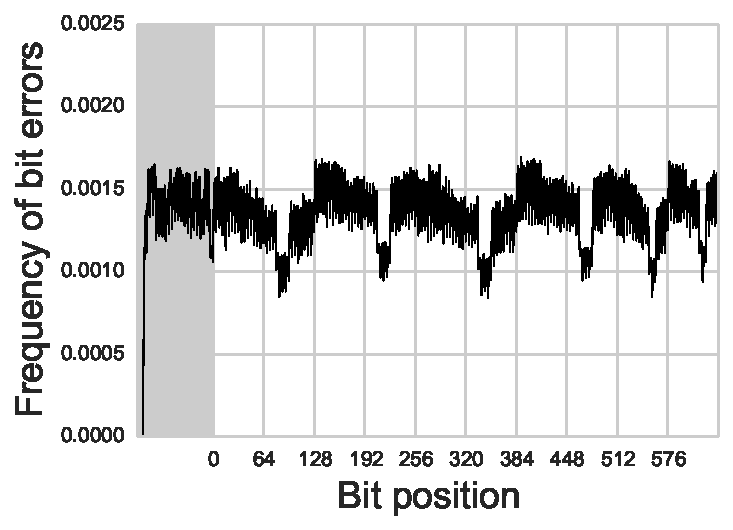
\includegraphics[width=0.475\columnwidth]{figures/8mote_2-7_xor_simulation}
		\label{fig:8mote_s_simulation}
	}
	\subfigure[Simulated XL burst error length.] {
		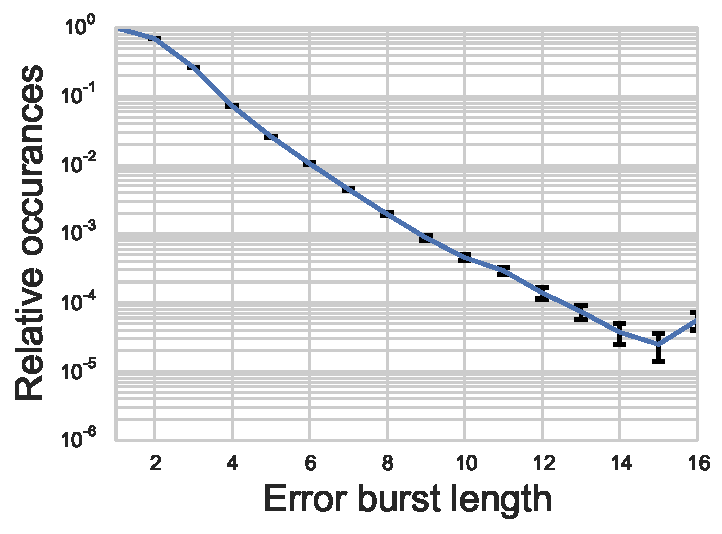
\includegraphics[width=0.475\columnwidth]{figures/8mote_0-5_burst_simulation}
		\label{fig:8mote_xl_burst_simulation}
	}
	\subfigure[Simulated S burst error length.] {
		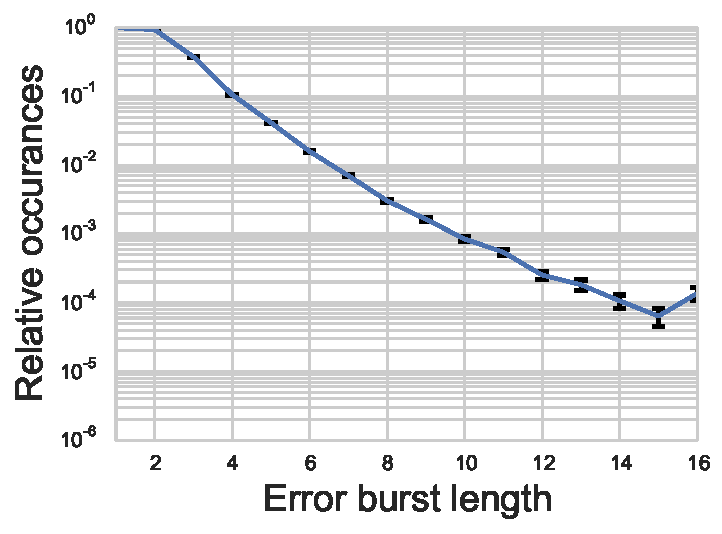
\includegraphics[width=0.475\columnwidth]{figures/8mote_2-7_burst_simulation}
		\label{fig:8mote_s_burst_simulation}
	}
	\caption{Error patterns of simulated constant payload using traces with constant payload. The error bars denote 99\% confidence intervals.}
	\label{fig:8mote_bit_errors_simulation}
\end{figure}

\paragraph{Packet Reception Rate}

To compare the overall number of corrupted messages of the original with the simulated link, we plotted the normalized \ac{PRR} of our original experiment with $RS(80,70)$ encoded payload and the simulation of that experiment with the same payload, as shown in Figures~\ref{fig:prr_link_01_fec} and \ref{fig:prr_link_10_fec} respectively.
To be able to compare the \ac{PRR} of encoded and non-encoded payload, we only evaluate the first $k=70$ bytes in the payload.
The timeouts shown in gray are the same for the simulation, since they are copied from the original, as mentioned before.

While the total amount of corrupted messages in the simulated link is the same as in the original link, as exemplified by the very similar error-free reception curves in the plots, error-free \ac{RS} decoded receptions yields slightly worse results, especially in areas with high byte error count, as visible in Figure~\ref{fig:prr_link_01_receiver_fec} and \ref{fig:prr_link_10_transmitter_fec}.
This shows that in these areas, the simulator overshoots the target bit error distribution of the original messages, and therefore undershoots the \ac{RS} decoded \ac{PRR} of the original link.
In the worst case, the simulated \ac{RS} performance is underestimated compared to reality, which is sufficient for our assessments.

\begin{figure}[t]
	\subfigure[Comparison of link~\ref{fig:prr_link_01_transmitter}.] {
		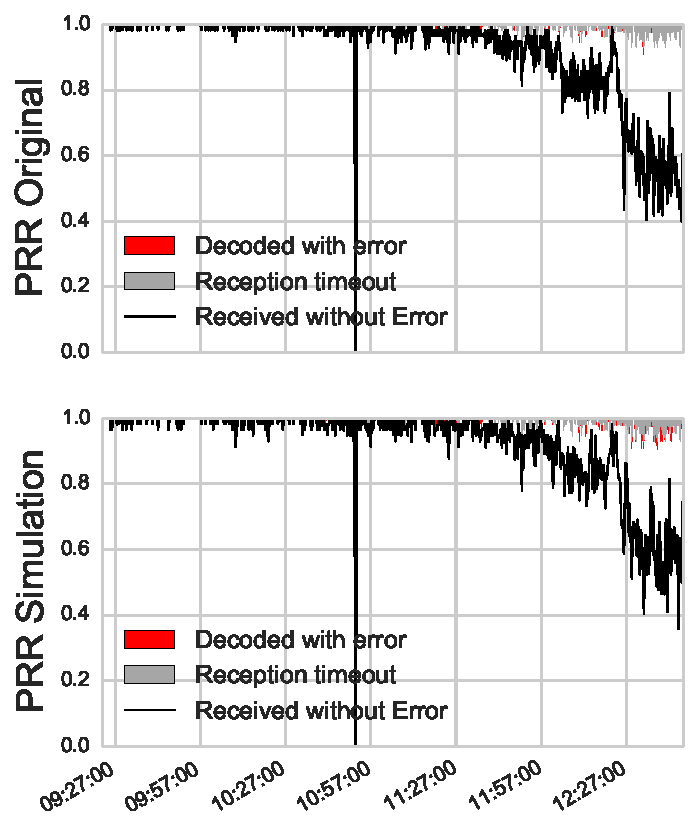
\includegraphics[width=0.475\columnwidth]{figures/fec_scheme_box0_box1_os_0-1_Throughput}
		\label{fig:prr_link_01_transmitter_fec}
	}
	\subfigure[Comparison of link~\ref{fig:prr_link_01_receiver}.] {
		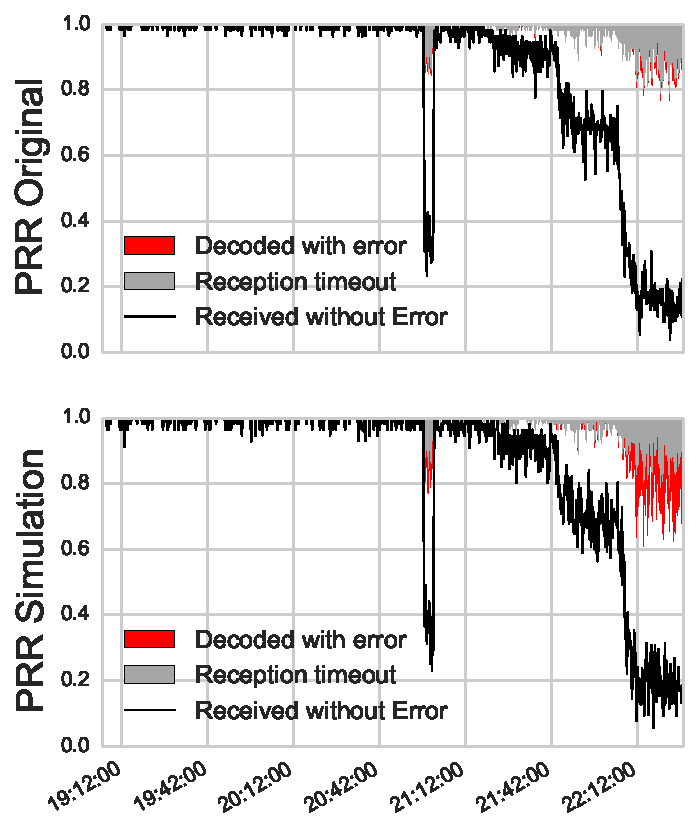
\includegraphics[width=0.475\columnwidth]{figures/fec_scheme_box1_box0_os_0-1_Throughput}
		\label{fig:prr_link_01_receiver_fec}
	}
	\caption{Original and simulated \acs{PRR} of the two $RS(80,70)$ encoded links of Figure~\ref{fig:prr_link_01}. Note the drop in simulated \acs{RS} decoded \acs{PRR} in (b).}
	\label{fig:prr_link_01_fec}
\end{figure}

\begin{figure}[t]
	\subfigure[Comparison of link~\ref{fig:prr_link_10_receiver}.] {
		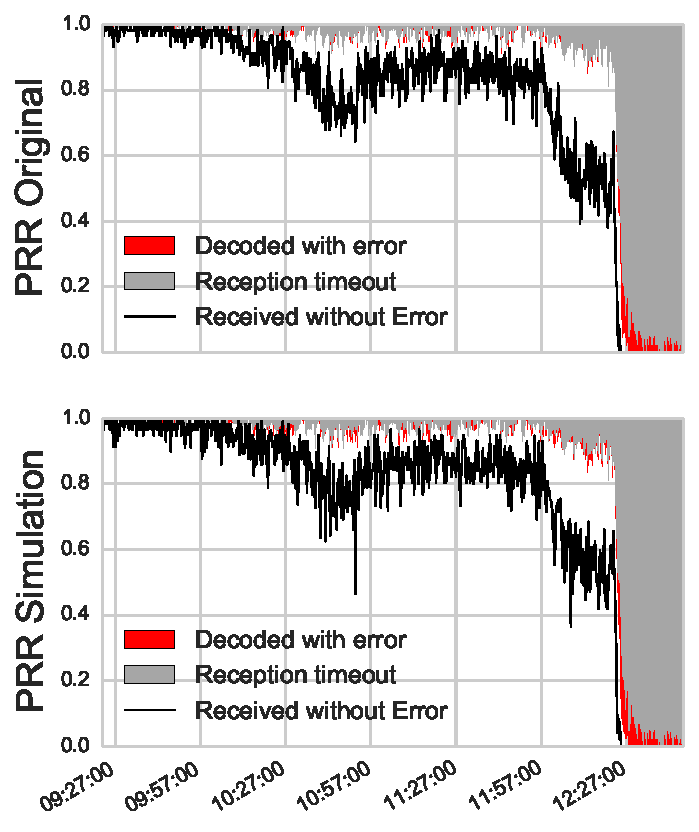
\includegraphics[width=0.475\columnwidth]{figures/fec_scheme_box0_box1_os_1-0_Throughput}
		\label{fig:prr_link_10_receiver_fec}
	}
	\subfigure[Comparison of link~\ref{fig:prr_link_10_transmitter}.] {
		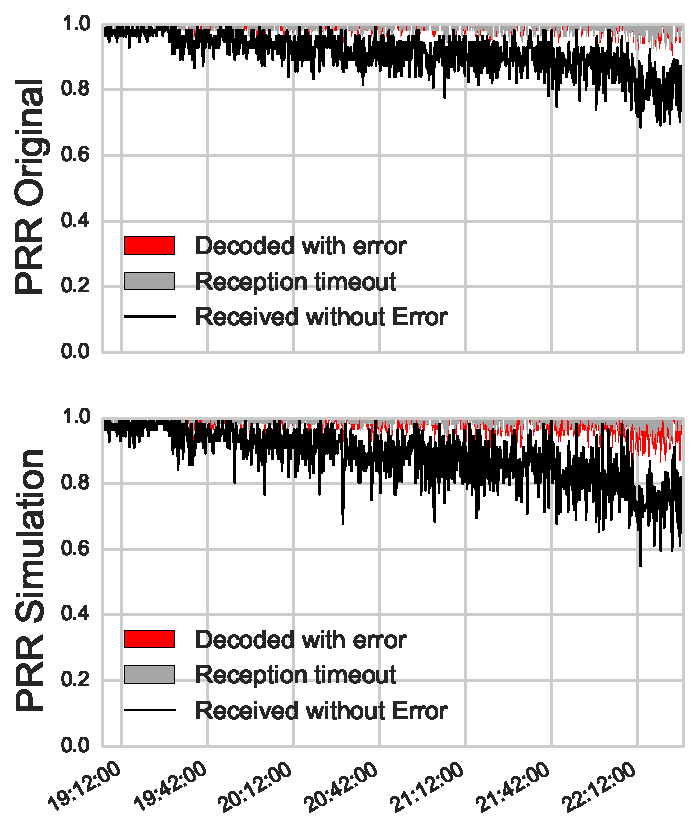
\includegraphics[width=0.475\columnwidth]{figures/fec_scheme_box1_box0_os_1-0_Throughput}
		\label{fig:prr_link_10_transmitter_fec}
	}
	\caption{Original and simulated \acs{PRR} of the two $RS(80,70)$ encoded links of Figure~\ref{fig:prr_link_10}.}
	\label{fig:prr_link_10_fec}
\end{figure}

These results show that this simple simulator is a very good time- and cost-saving alternative to testing the effects of different payloads over a real link, if good original data is available.
Using our trace-based simulator eliminates the effect of uncontrollable environmental factors or hardware issues on repeatability and allows us to focus purely on the message content, without assuming  idealized and monolithic link properties.


\section{Comparing \acs{RS} Scheme Strengths}

Our first idea was to keep a constant data size of $k=80$ and add parity bytes, making the entire message longer.
However, longer packets require more energy to transmit, a metric which has to be included somehow when comparing different $k$.
Furthermore, because of the size limit of the \ac{MPDU} of 127 bytes, of which 26 are already used, this only leaves $n=101$ bytes with a maximum of $n-k=19$ parity bytes, which would not allow to encode with more than 18\% coding overhead.
We could have split the message into two packets, however, this would have made it even harder to compare them, since now two packets must be received in the right sequence.

Therefore, we abandoned this idea and fit the entire encoded message into 80 bytes, including parity bytes as shown in Figure~\ref{fig:rs_codeword}.
This means we can only transfer $k$ bytes of encoded data, effectively reducing data rate while gaining robustness, which we want to use for a metric for comparing \ac{RS} performance.
We combine this reduction of data rate and the corruption of decoded packets as throughput, normalized over the number of \emph{received} messages.
We calculated the normalized throughput $T(80, k)$ using the following formula:

\[ T(80, k) = \frac{k}{80} \frac{PRR_{decoded}}{PRR_{received}} \]

This metric allows us to compare \ac{RS} performance not only between different coding strengths, but augment that comparison with context of the link's quality.
% The normalized throughputs of the original versus simulated links are also available in Figures~\ref{fig:prr_link_01_fec} and \ref{fig:prr_link_10_fec}.
% Especially the drop in Figure~\ref{fig:prr_link_01_receiver} visualizes the previous findings that the simulation slightly underestimates, but never overestimates \ac{RS} decoded \ac{PRR}.

For each of the four links discussed in Section~\ref{sec:packet_reception_rate} we simulated new $RS(80, k)$ encoded payload for $k$ in 10 byte increments up to $k=60$, then in 2 byte increments up to $k=78$.
We plotted the normalized throughputs $T(80, k)$ in Figure~\ref{fig:throughput_link_fec}, with the dashed line showing throughput without RS encoding.
The graphs illustrate that even using only 2 parity bytes at $k=78$ can already significantly improve \ac{PRR}, since most messages only have a few burst errors, and all those constrained to one byte can be corrected.

Adding two more parity bytes for $k=76$ improves \ac{PRR} even more, but only in a few areas.
From $k=74$ to $k=60$ no significant improvement shows, especially at low temperatures.
Using $k=60$ shows stability up to high temperature of $80\,^{\circ}\mathrm{C}$ in all Figures except \ref{fig:throughput_link_10_receiver_fec}.
At and below $k=50$ no improvement of throughput is visible except in Figure~\ref{fig:throughput_link_10_receiver_fec}, where $k=30$ and $k=20$ hold throughput the longest.

By comparing Figure~\ref{fig:prr_link_01_receiver_fec} and \ref{fig:throughput_link_01_receiver_fec}, we can deduct that in that link the simulated throughput above \SI{70}{\celsius} is actually worse than in reality. Therefore we can safely assume $k=60$ as stable at that temperature.

\begin{figure}[t]
	\subfigure[Simulated link~\ref{fig:prr_link_01_transmitter}.] {
		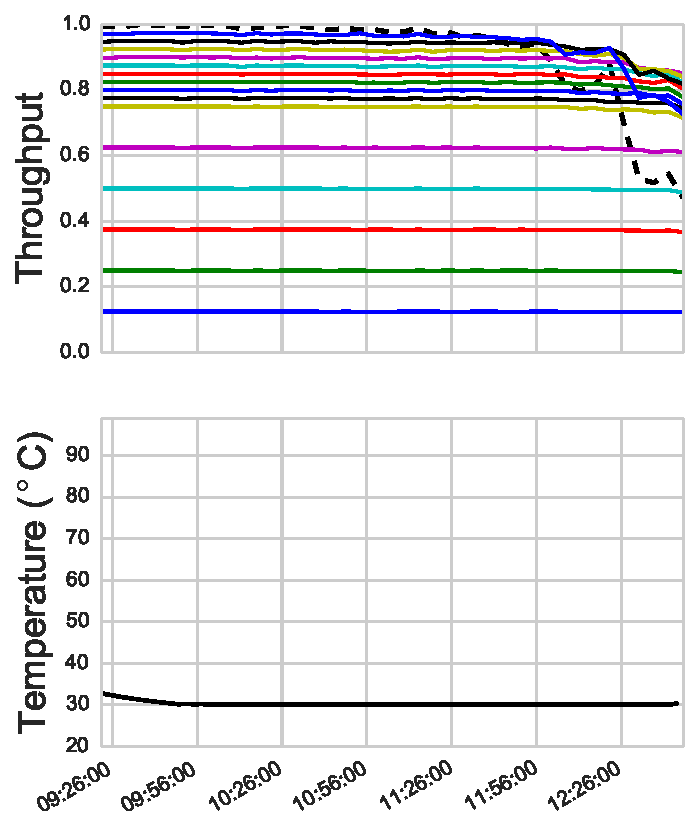
\includegraphics[width=0.475\columnwidth]{figures/fec_scheme_box0_box1_0-1_Throughput}
		\label{fig:throughput_link_01_transmitter_fec}
	}
	\subfigure[Simulated link~\ref{fig:prr_link_01_receiver}.] {
		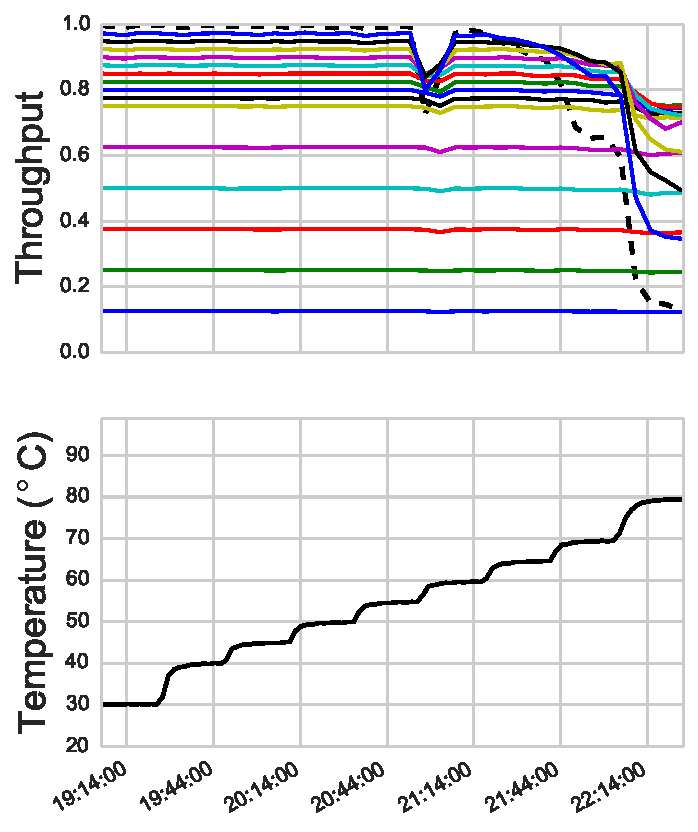
\includegraphics[width=0.475\columnwidth]{figures/fec_scheme_box1_box0_0-1_Throughput}
		\label{fig:throughput_link_01_receiver_fec}
	}
	\subfigure[Simulated link~\ref{fig:prr_link_10_receiver}.] {
		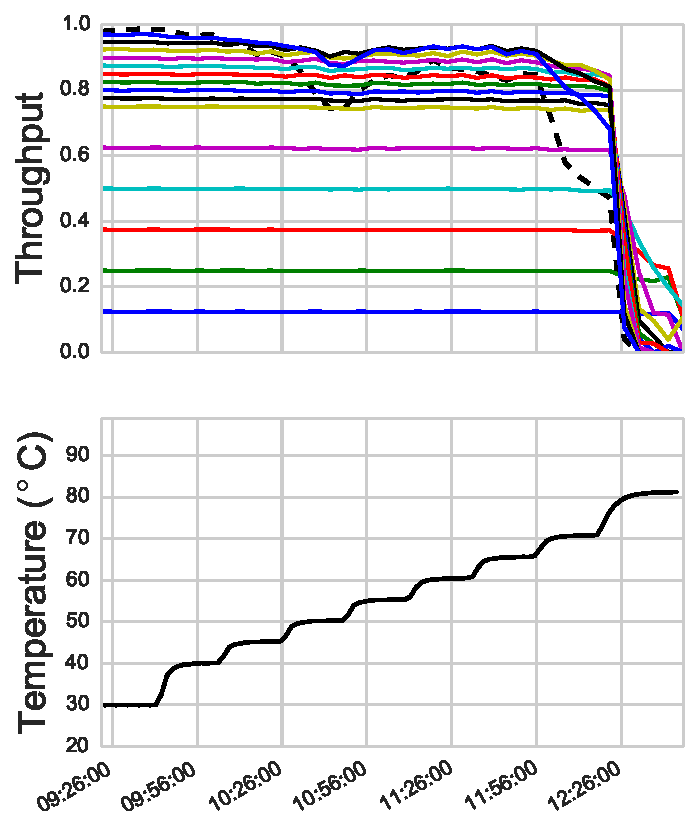
\includegraphics[width=0.475\columnwidth]{figures/fec_scheme_box0_box1_1-0_Throughput}
		\label{fig:throughput_link_10_receiver_fec}
	}
	\subfigure[Simulated link~\ref{fig:prr_link_10_transmitter}.] {
		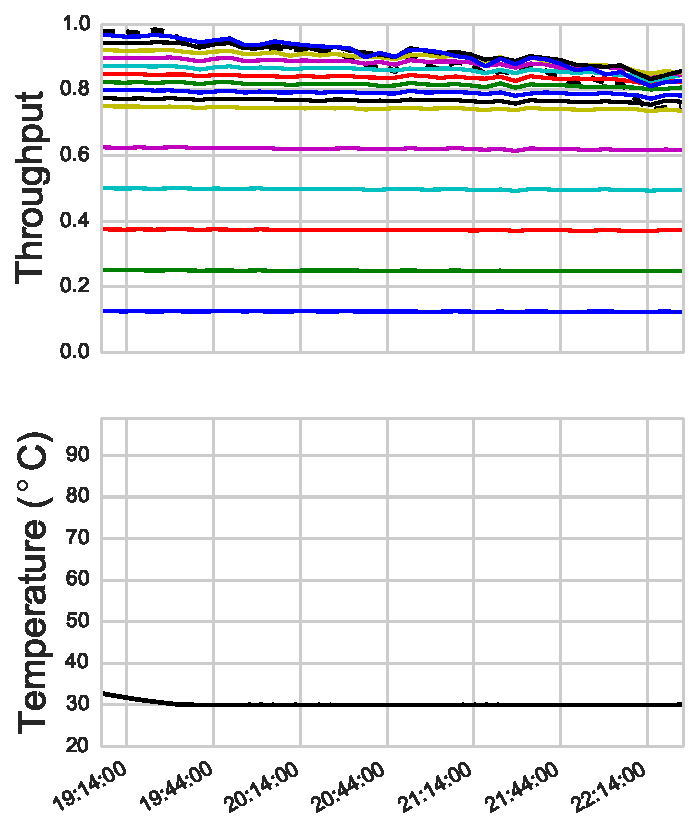
\includegraphics[width=0.475\columnwidth]{figures/fec_scheme_box1_box0_1-0_Throughput}
		\label{fig:throughput_link_10_transmitter_fec}
	}
	\caption{Comparison of throughputs $T(80, k)$ of all four simulated links of Section~\ref{sec:packet_reception_rate} for \\$k \in \{10,20,30,40,50,60,62,64,66,68,70,72,74,76,78\}$ over temperature. The dashed line shows throughput at $k=80$, which is equivalent to using no parity bytes.}
	\label{fig:throughput_link_fec}
\end{figure}



\section{Discussion}

Considering that the goal of using an \ac{FEC} in the context of low power networks such as \ac{WSN}s is to maximize energy efficiency of communications, we are not only looking for the $k$ with maximum throughput, but also with the least retransmissions.
We also have to consider that the link quality can already be poor at low temperature, therefore using no parity bytes at low temperatures is not a good idea either.

As per our findings, we propose one possible \ac{RS} scheme starting with $k=70$, which is 12.5\% overhead (the same as the popular $RS(255,223)$~\cite{Ma2009}), at low temperatures and linearly increase this to $k=60$ (or 25\% overhead) as receiver temperature increases to $70\,^{\circ}\mathrm{C}$ and above.
Starting with $k=70$ will give some protection against a random decrease in link quality as seen in Figure~\ref{fig:throughput_link_01_receiver_fec}.
In cases of extremely high bit error, such as in Figure~\ref{fig:throughput_link_10_receiver_fec}, we can still regain some throughput by using $60-80\%$ coding overhead with $k=30$ or $k=20$.
However, considering the extremely low \ac{PRR} in this area (compare with Figure~\ref{fig:prr_link_10_receiver_fec}), most of these messages will likely never be received anyway, which makes this option only viable when communication at these temperatures is absolutely necessary.

The results of Boano~\etal~\cite{Boano2013} strongly suggested that the loss in \ac{PRR} is more pronounced when heating the transmitter than the receiver.
This would have allowed us to use local temperature measurements to adapt the coding strength of our \ac{FEC} scheme to counteract the loss in \ac{PRR}.
Unfortunately, our results firmly oppose the findings of Boano~\etal{}: heating the receiver creates a higher loss in \ac{PRR} than heating the transmitter, therefore making such an approach unusable.
However, using temperature as another source for assessing link quality has the distinct advantage of being always available on the receiver locally, compared to \ac{LQI} and \ac{RSSI}, which requires a message to be received first.

We therefore propose another solution to adapt \ac{FEC} strength:
the receiver should monitor its local temperature and send out a warning broadcast to all potential transmitters, before its temperature becomes too high.
The transmitters can then address this mote with the appropriate \ac{FEC} strength.
The advantage of this active, preemptive approach over backchanneling link quality information is that in setups where transmissions only occur sparsely, a ``test'' transmission to judge link quality is not required.



